%%%%%%%%%%%%%%%%%%%%%%%%%%%%%%%%%%%%%%%%%%%%%%%%%%%%%%%%%%%%%%%%%%
%%%%%%%%%%%%%%%%%%%%%%%%%%%%%%%%%%%%%%%%%%%%%%%%%%%%%%%%%%%%%%%%%%
%Packages
\documentclass[10pt, a4paper]{article}
\usepackage[UTF8]{ctex}
\usepackage[top=3cm, bottom=4cm, left=3.5cm, right=3.5cm]{geometry}
\usepackage{amsmath,amsthm,amsfonts,amssymb,amscd, fancyhdr, color, comment, graphicx, environ}
\usepackage{float}
\usepackage{mathrsfs}
\usepackage[math-style=ISO]{unicode-math}
\setmathfont{TeX Gyre Termes Math}
\usepackage{lastpage}
\usepackage[dvipsnames]{xcolor}
\usepackage[framemethod=TikZ]{mdframed}
\usepackage{enumerate}
\usepackage[shortlabels]{enumitem}
\usepackage{fancyhdr}
\usepackage{indentfirst}
\usepackage{listings}
\usepackage{sectsty}
\usepackage{thmtools}
\usepackage{shadethm}
\usepackage{hyperref}
\usepackage{CJKfntef}
\usepackage{setspace}
\hypersetup{
    colorlinks=true,
    linkcolor=blue,
    filecolor=magenta,      
    urlcolor=blue,
}
%%%%%%%%%%%%%%%%%%%%%%%%%%%%%%%%%%%%%%%%%%%%%%%%%%%%%%%%%%%%%%%%%%
%%%%%%%%%%%%%%%%%%%%%%%%%%%%%%%%%%%%%%%%%%%%%%%%%%%%%%%%%%%%%%%%%%
%Environment setup
\mdfsetup{skipabove=\topskip,skipbelow=\topskip}
\newrobustcmd\ExampleText{%
An \textit{inhomogeneous linear} differential equation has the form
\begin{align}
L[v ] = f,
\end{align}
where $L$ is a linear differential operator, $v$ is the dependent
variable, and $f$ is a given non−zero function of the independent
variables alone.
}
\mdfdefinestyle{theoremstyle}{%
linecolor=black,linewidth=1pt,%
frametitlerule=true,%
frametitlebackgroundcolor=gray!20,
innertopmargin=\topskip,
}
\mdtheorem[style=theoremstyle]{Problem}{作业题}
\newenvironment{Solution}{}

%%%%%%%%%%%%%%%%%%%%%%%%%%%%%%%%%%%%%%%%%%%%%%%%%%%%%%%%%%%%%%%%%%
%%%%%%%%%%%%%%%%%%%%%%%%%%%%%%%%%%%%%%%%%%%%%%%%%%%%%%%%%%%%%%%%%%
%Fill in the appropriate information below
\newcommand{\norm}[1]{\left\lVert#1\right\rVert}     
\newcommand\course{最优化方法}                         % <-- course name   
%\newcommand\hwnumber{1}                              % <-- homework number
\newcommand\Information{李邹/人工智能一班}          % <-- personal information
%%%%%%%%%%%%%%%%%%%%%%%%%%%%%%%%%%%%%%%%%%%%%%%%%%%%%%%%%%%%%%%%%%
%%%%%%%%%%%%%%%%%%%%%%%%%%%%%%%%%%%%%%%%%%%%%%%%%%%%%%%%%%%%%%%%%%
%Page setup
\pagestyle{fancy}
\headheight 35pt
\lhead{\today}
\rhead{
\includegraphics[width=2.5cm]{lzu-logo.png}}
\lfoot{}
\pagenumbering{arabic}
\cfoot{\small\thepage}
\rfoot{}
\headsep 1.2em
\renewcommand{\baselinestretch}{1.25}
%%%%%%%%%%%%%%%%%%%%%%%%%%%%%%%%%%%%%%%%%%%%%%%%%%%%%%%%%%%%%%%%%%
%%%%%%%%%%%%%%%%%%%%%%%%%%%%%%%%%%%%%%%%%%%%%%%%%%%%%%%%%%%%%%%%%%
%Add new commands here
\renewcommand{\labelenumi}{\alph{enumi})}
\newcommand{\Z}{\mathbb Z}
\newcommand{\R}{\mathbb R}
\newcommand{\Q}{\mathbb Q}
\newcommand{\NN}{\mathbb N}
\DeclareMathOperator{\Mod}{Mod} 
\renewcommand\lstlistingname{Algorithm}
\renewcommand\lstlistlistingname{Algorithms}
\def\lstlistingautorefname{Alg.}
%%%%%%%%%%%%%%%%%%%%%%%%%%%%%%%%%%%%%%%%%%%%%%%%%%%%%%%%%%%%%%%%%%
%%%%%%%%%%%%%%%%%%%%%%%%%%%%%%%%%%%%%%%%%%%%%%%%%%%%%%%%%%%%%%%%%%
%Begin now!



\begin{document}

\begin{titlepage}
    \begin{center}
        \vspace*{3.5cm}
            
        \Huge
        \textbf{作业11}
            
        \vspace{2cm}
        \LARGE
        李邹
            
        \vspace{0.1cm}
        \Large
        人工智能一班(2020级)                      % <-- author
        
            
        \vfill
        
        \course \ 课程作业
            
        \vspace{1cm}
            
        
\includegraphics[width=0.4\textwidth]{lzu-logo.png}
        \\
        
        \Large
        
        \today
            
    \end{center}
\end{titlepage}

%%%%%%%%%%%%%%%%%%%%%%%%%%%%%%%%%%%%%%%%%%%%%%%%%%%%%%%%%%%%%%%%%%
%%%%%%%%%%%%%%%%%%%%%%%%%%%%%%%%%%%%%%%%%%%%%%%%%%%%%%%%%%%%%%%%%%
%Start the assignment now

%%%%%%%%%%%%%%%%%%%%%%%%%%%%%%%%%%%%%%%%%%%%%%%%%%%%%%%%%%%%%%%%%%
%New problem
\newpage
\begin{Problem}
    \textbf{一个简单的例子。}\;考虑优化问题
    $$
    \begin{array}{ll}
    \operatorname{minimize} & x^{2}+1  \\
    \text {subject to } & (x-2)(x-4) \le 0 \\
    \end{array}
    $$
    其中变量$x\in \textbf{R}$
    \begin{enumerate}[(a)]
       \item \textbf{分析原问题。}求解可行集,最优值以及最优解。
       \item \textbf{Lagrange函数以及对偶函数。}绘制目标函数根据$x$变化的图像。在同一幅图中,标出可行集,最优点及最优值,选择一些正的Lagrange乘子$\lambda $,绘出Lagrange函数$L(x,\lambda)$关于$x$的变化曲线。利用图像,证明下界性质(对任意$\lambda \ge 0,p^{*} \ge inf_{x}L(x,\lambda)$)。推导Lagrange对偶函数$g$并大致描绘其图像。
       \item \textbf{Lagrange对偶问题。}描述对偶问题,证明它是一个凹极大化问题。求解对偶最优值以及对偶最优解$\lambda^{*}$。此时强对偶性是否成立?
    \end{enumerate}
\end{Problem}
    
\begin{Solution}
\textbf{解答}
\end{Solution}
%Complete the assignment now
\begin{enumerate}[(a)]
    \item 由不等式约束可知,可行集为$x\in \left [ 2,4 \right ] $,令$f(x)=x^{2}+1$,问题可转化为求解
    \[f_{min}(x)=x^{2}+1,x\in \left [ 2,4 \right ]\]

    对$f(x)$求导,可得${f_{0}}'(x) =2x$,其在定义域上单调递增。所以有$f_{min}(2)=5$.

    因此原优化问题在最优解$x=2$处取得最优值$p^{*}=5$.
    \item 目标函数根据$x$变化的图像如图1所示,其中可行集为两色块重合的区域,最优解与最优值已标出。
    \begin{figure}[H]
        \centering
        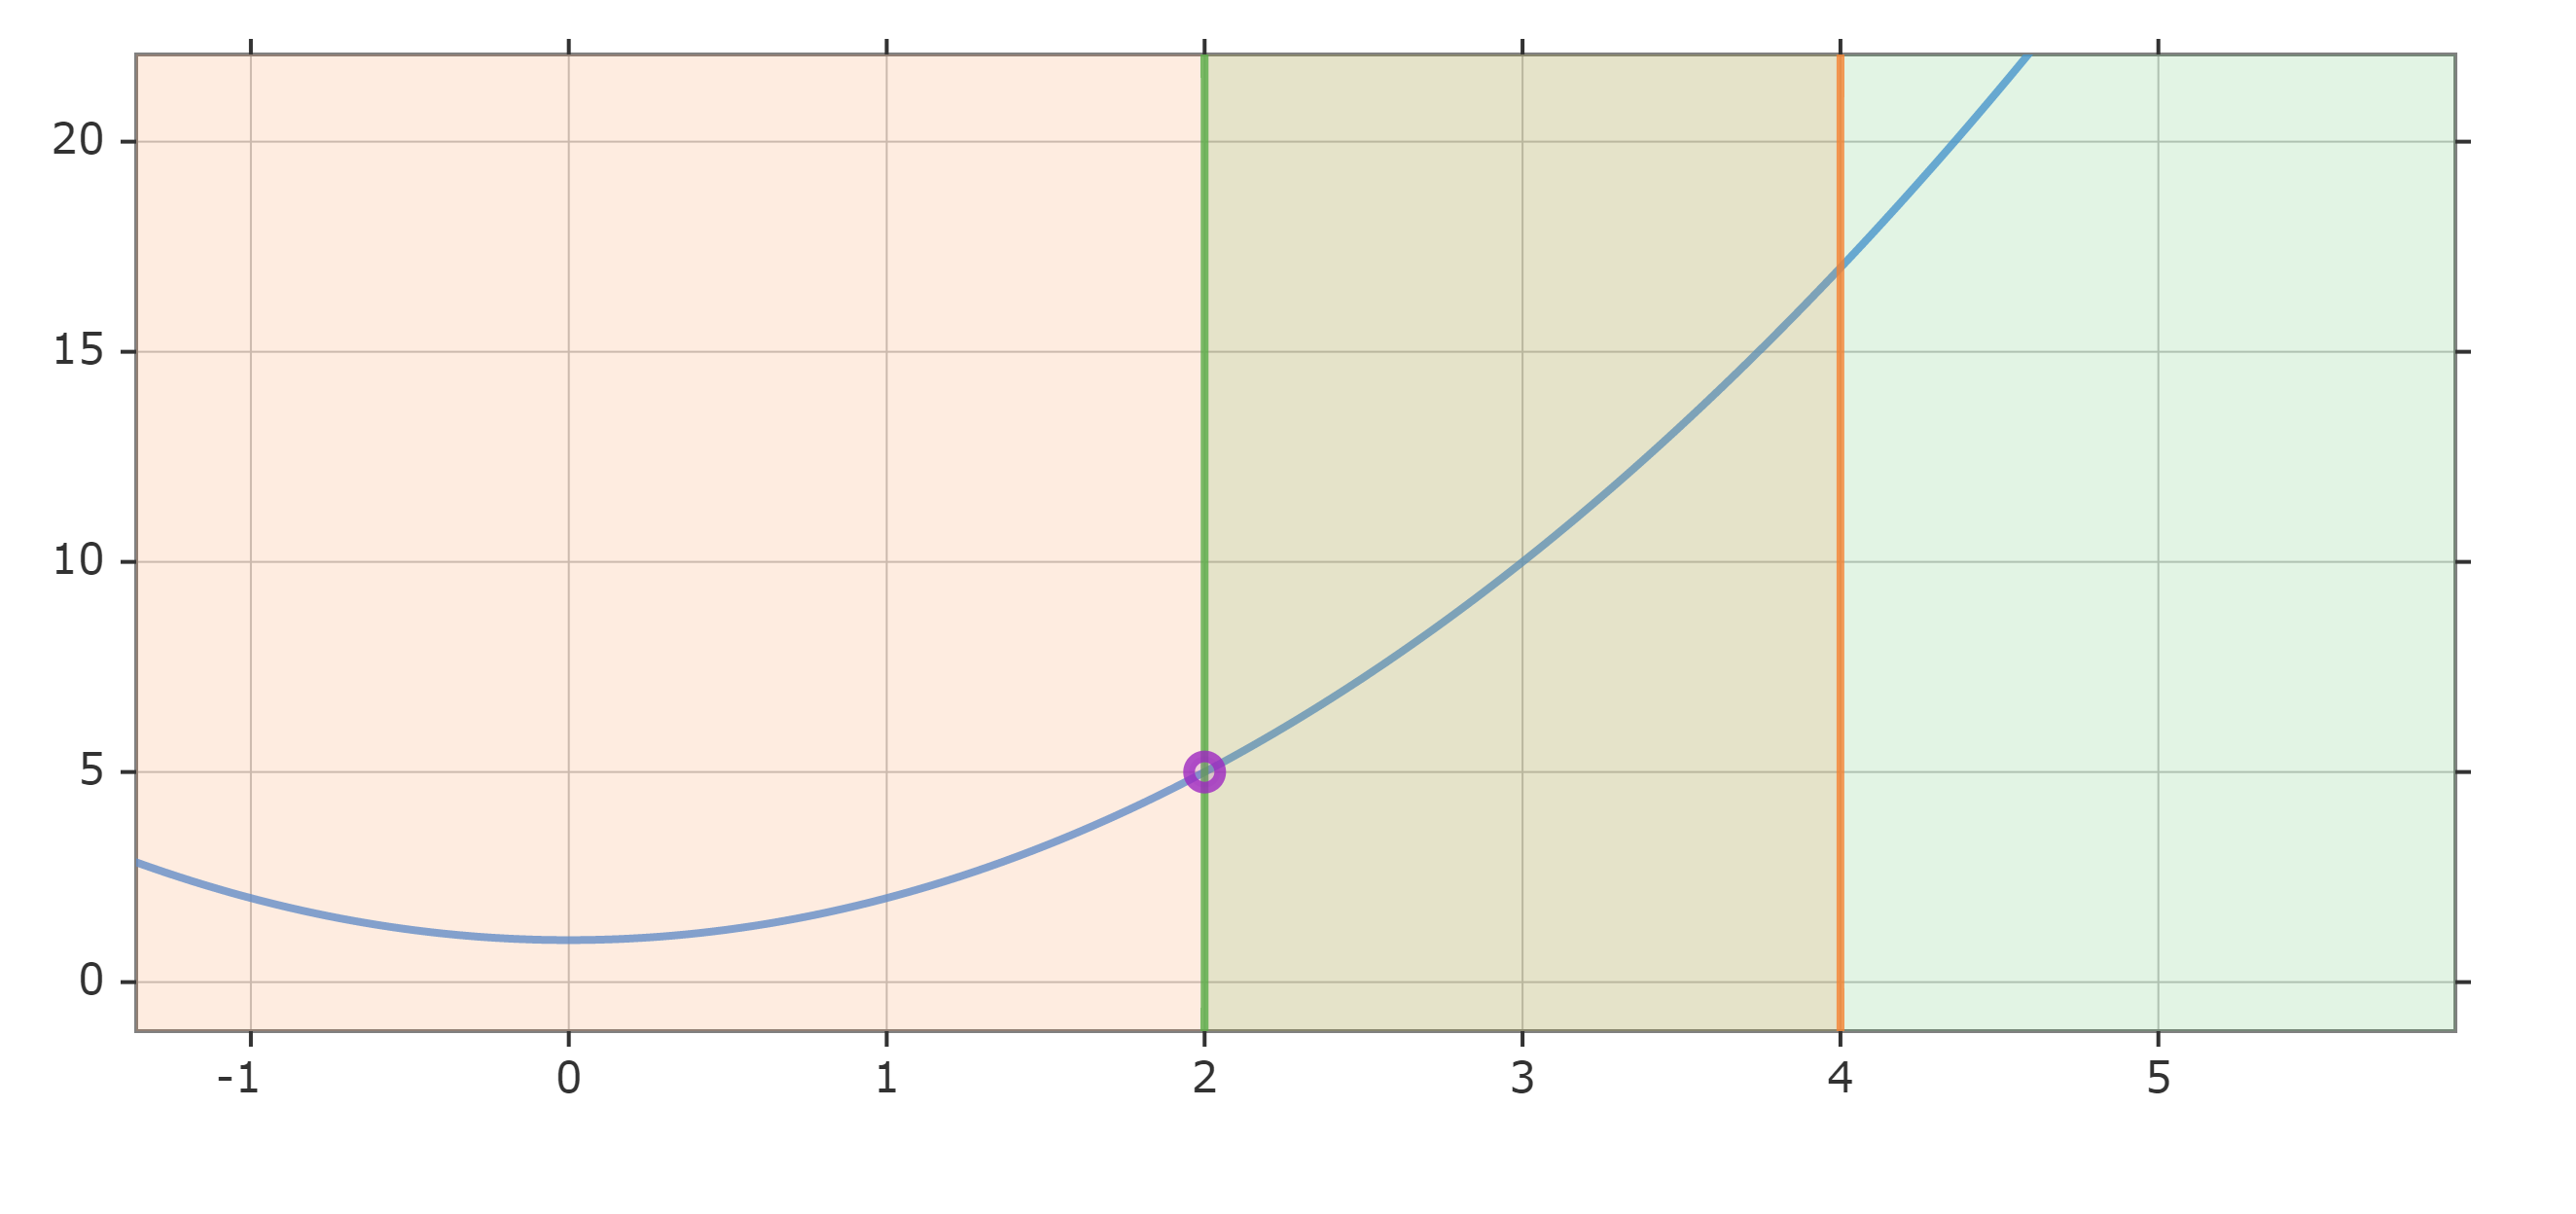
\includegraphics[scale=0.13]{1.png}
        \caption{目标函数图像}
    \end{figure}
    令$f_{0}(x)=x^{2}+1,f_{1}(x)=(x-2)(x-4)$,设$L_{i}(x)=f_{0}(x)+if_{1}(x)$.

    从而有$L(x, \lambda)=(1+\lambda) x^{2}-6 \lambda x+(1+8 \lambda)$.
    
    下图2是$\lambda$取$0,1,2,3$情况下的函数图像。
    \begin{figure}[H]
        \centering
        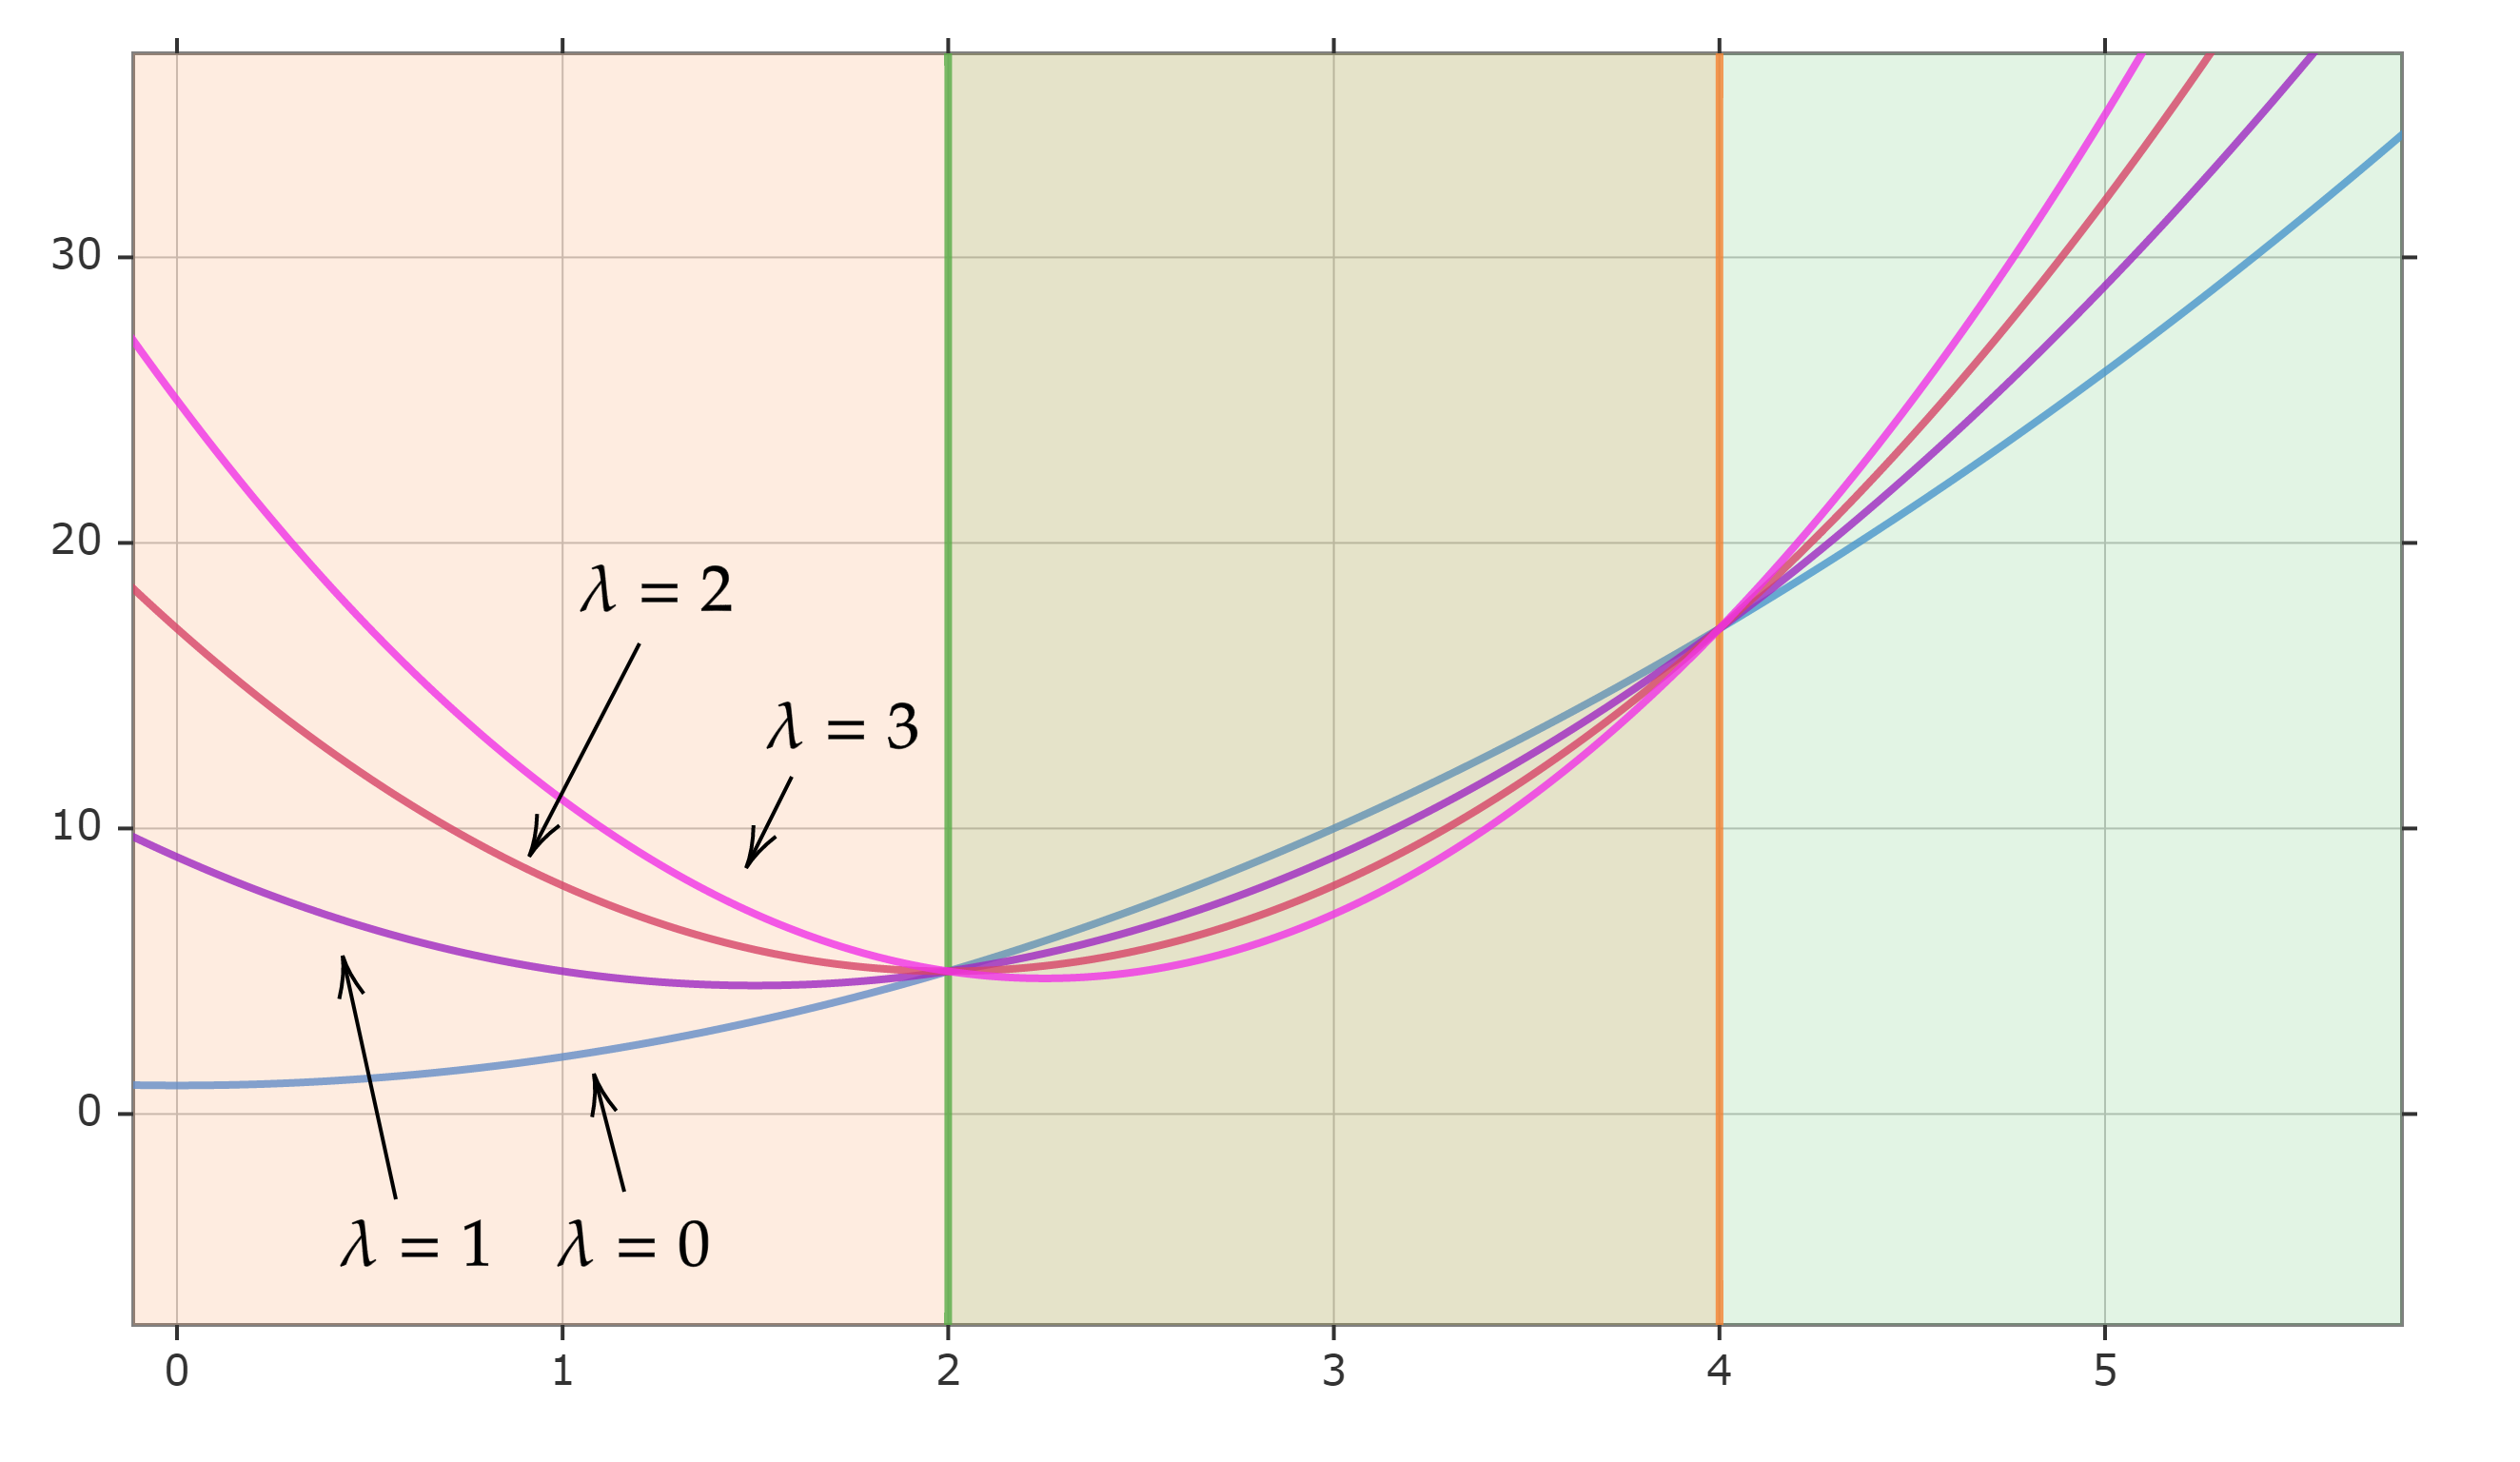
\includegraphics[scale=0.13]{2.png}
        \caption{$\lambda$不同取值下的函数图像}
    \end{figure}
    由图像可知,当$\lambda \ge 0$时,$inf_{x}L(x,\lambda) \leq 5$恒成立。
    
    因此我们可以证得,对于任意的$\lambda \ge 0,p^{*} \ge inf_{x}L(x,\lambda)$恒成立。

    将$L(x, \lambda)$做数学变换,可以得到
    \[L_{\lambda}(x)=(1+\lambda )(x-\frac{3\lambda }{1+\lambda } ) ^{2} -\frac{9\lambda ^{2} }{1+\lambda } +8\lambda +1\]

    所以,当$\lambda > -1$时,$L_{\lambda}(x)$在$x=\frac{3\lambda }{1+\lambda }$处取得下确界,否则下确界不存在。

    因此我们得到其对偶函数
    \begin{align}
        g(\lambda) & = \begin{cases}
          -\frac{9\lambda ^{2} }{1+\lambda } +8\lambda +1&  x >-1 \\
          -\infty &  x \le -1
        \end{cases}
    \end{align}

    其图像如图3所示。
    \begin{figure}[H]
        \centering
        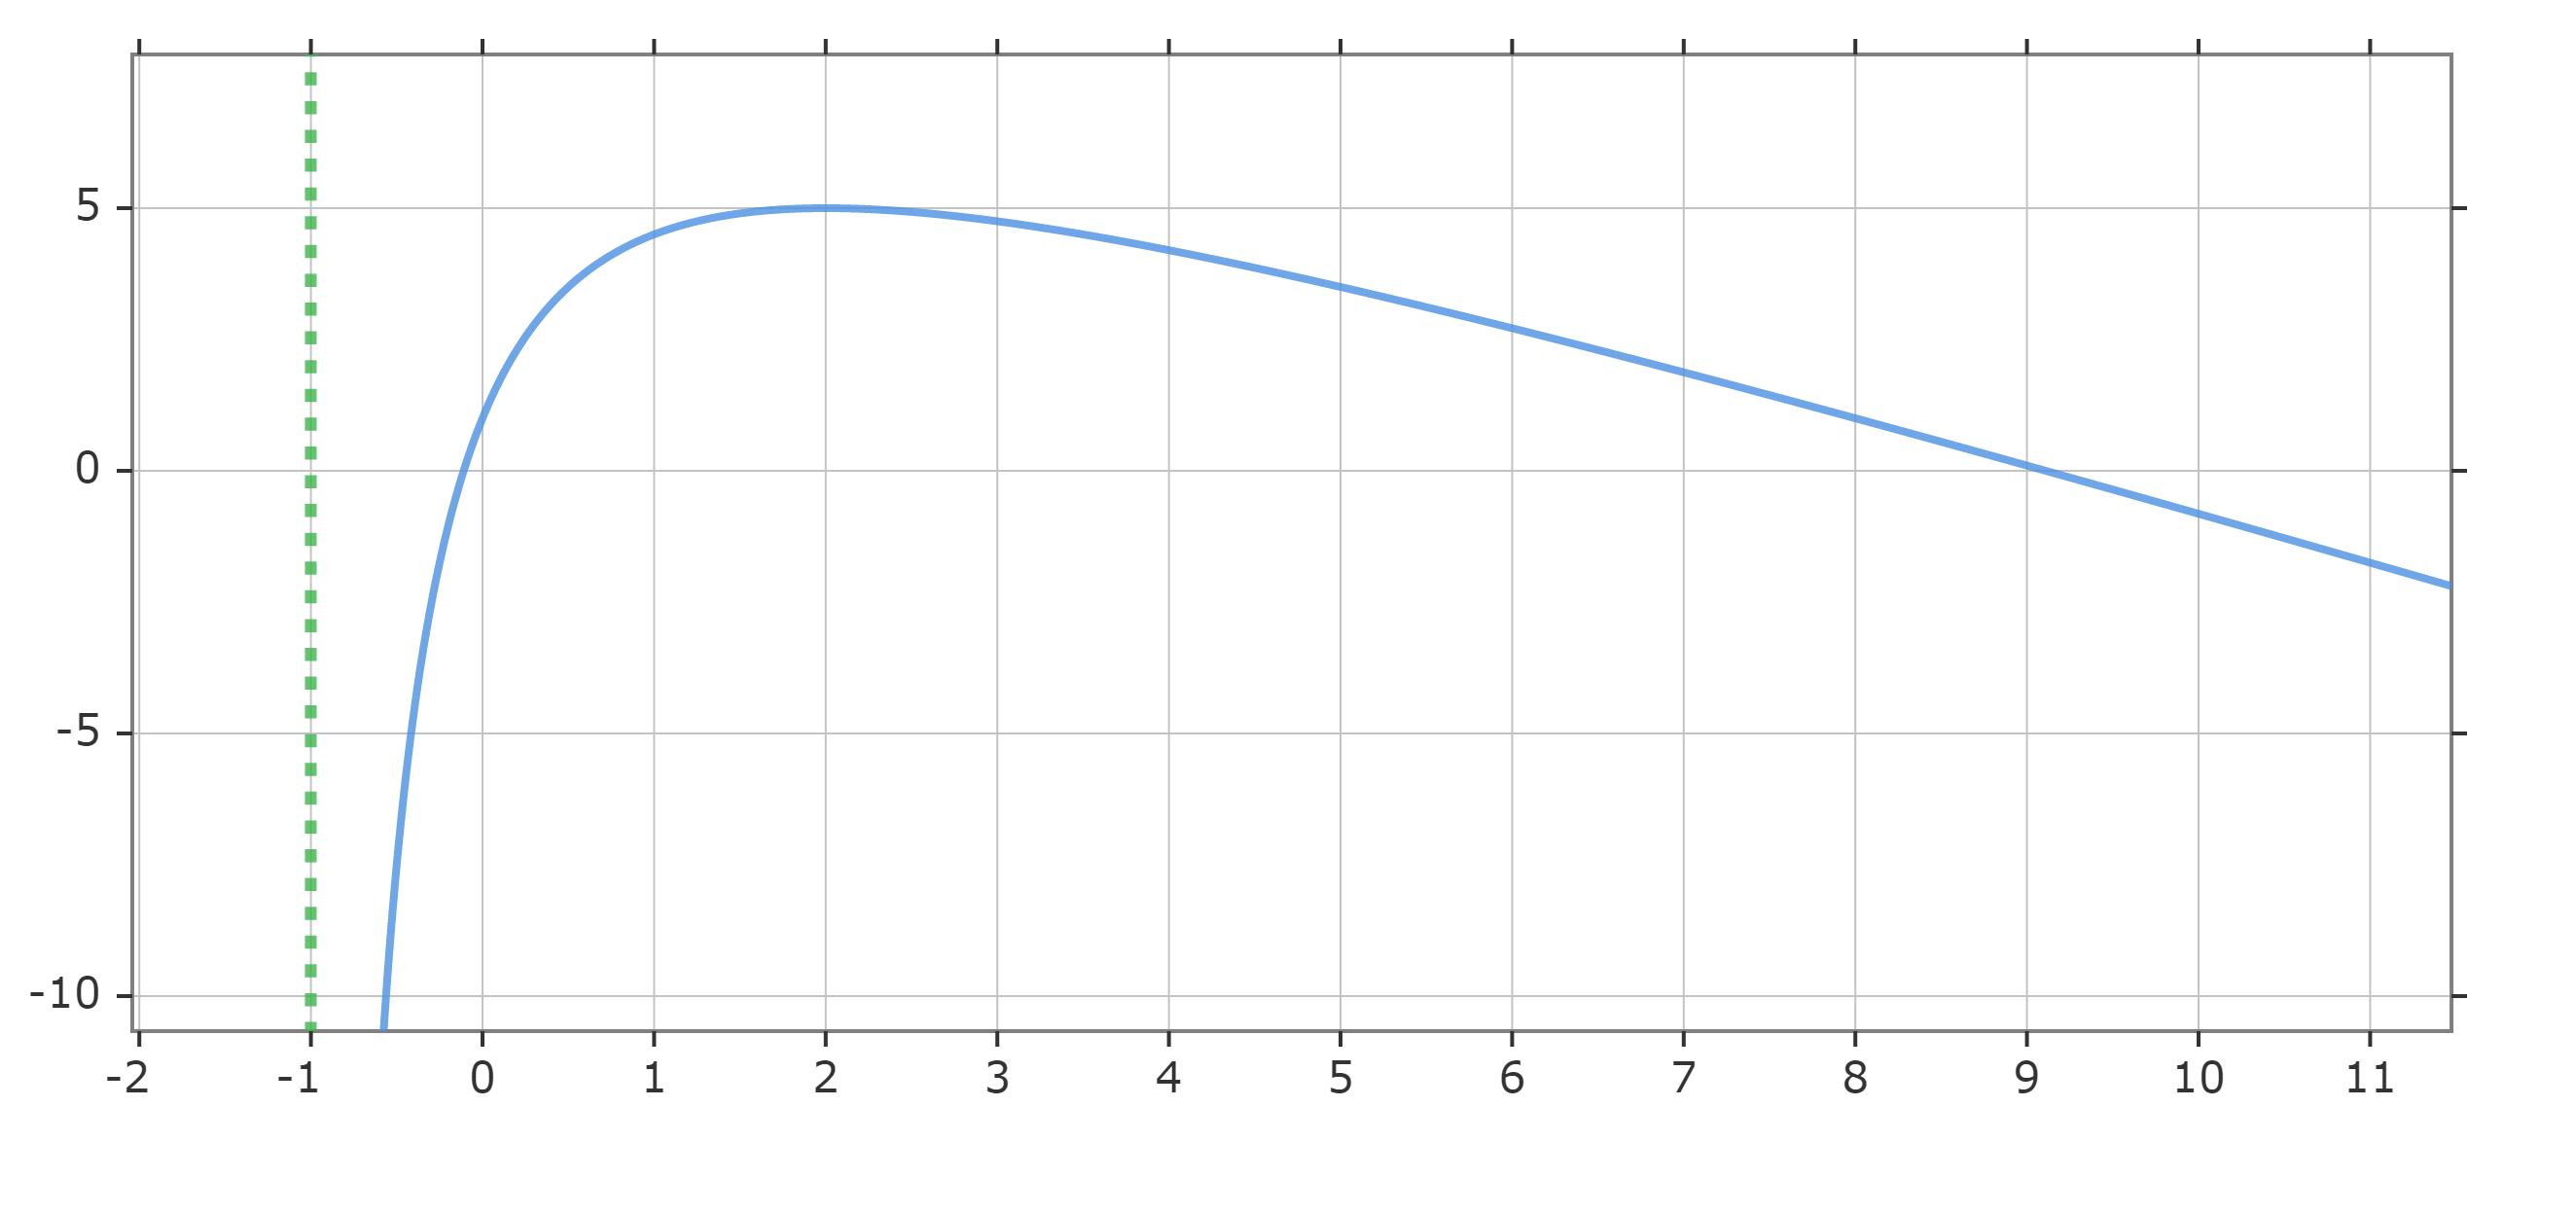
\includegraphics[scale=0.13]{3.png}
        \caption{对偶函数图像}
    \end{figure}

    \item 将该问题描述成对偶问题为
    $$
    \begin{array}{ll}
    \operatorname{maximize} & -\frac{9\lambda ^{2} }{1+\lambda } +8\lambda +1  \\
    \text {subject to } & \lambda > 0 \\
    \end{array}
    $$

    由对偶函数定义可知,目标函数为凹函数,而不等式条件为$\lambda >0$,因此可得该问题转换为一个凹极大化问题。

    通过导数工具容易求解,当$\lambda=5$时取得最优值5,此时最优解$\lambda^{*}=2$,强对偶性成立。
\end{enumerate}

\hfill $\Box$
\vspace*{3em}


\end{document}

%%%%%%%%%%%%%%%%%%%%%%%%%%%%%%%%%%%%%%%%%%%%%%%%%%%%%%%%%%%%%%%%%%
%%%%%%%%%%%%%%%%%%%%%%%%%%%%%%%%%%%%%%%%%%%%%%%%%%%%%%%%%%%%%%%%%%
